%----------------------------------------------------------------------------------------
%	PACKAGES AND DOCUMENT CONFIGURATIONS
%----------------------------------------------------------------------------------------
\documentclass[article, a4paper, 12pt, oneside]{memoir}

% Margins
\usepackage[top=3cm,left=2cm,right=2cm,bottom=3cm]{geometry}

% Encondings
\usepackage[utf8]{inputenc}

% Language
\usepackage[portuguese]{babel}

% Graphics and images
\usepackage{graphicx}
	\graphicspath{{images/}}

% Tables
\usepackage{tabularx}

% Paragraph Spacing
\usepackage{parskip}
\usepackage{indentfirst}
\setlength{\parskip}{0.5cm}

% Hyperreferences
\usepackage{hyperref}

% Repeated commands
\usepackage{expl3}
\ExplSyntaxOn
\cs_new_eq:NN \Repeat \prg_replicate:nn
\ExplSyntaxOff

% Header and Footer Things
\usepackage{wallpaper}
\usepackage{fancyhdr}

% Following code to edit the pagestyle
\pagestyle{fancy}
\fancyhf{}
\rhead{WasteApp}
\lhead{\leftmark}
\rfoot{Página \thepage}

% Commands
\usepackage{xargs}

%% Linked Email
\newcommand{\email}[1]{
{\textup{\href{mailto:#1}{#1}} }
}

%----------------------------------------------------------------------------------------
%	DOCUMENT INFORMATION
%----------------------------------------------------------------------------------------
% Title
\title{\Huge \textup{WasteApp: recolha seletiva de lixo (Parte 1)} }
% Authors
\author{
\LARGE \textbf{Turma 1 - Grupo 1}\\\\
\begin{tabular}{l r}
	\email{up201806551@fe.up.pt} & Beatriz Costa Silva Mendes				\\
	\email{up201806524@fe.up.pt} & Daniel Garcia Lima Sarmento da Silva		\\
	\email{up201806538@fe.up.pt} & Henrique Manuel Ruivo Pereira			\\
	\Repeat{4}{\linebreak}
\end{tabular}
}

%\institute{Faculdade de Engenharia da Universidade do Porto \\ Concepção e Análise de Algoritmos - Turma 1, grupo 1}

% Date for the report
\date{24 de abril de 2020}

% Table of Contents
\addto\captionsportuguese{\renewcommand*\contentsname{Índice}}

%----------------------------------------------------------------------------------------
%	DOCUMENT
%----------------------------------------------------------------------------------------
\begin{document}
%----------------------------------------------------------------------------------------
%	Front Page
%----------------------------------------------------------------------------------------
% Title Author and Date
\maketitle

% More information for front page
\begin{center}
\textbf{Projeto CAL - 2019/20 - MIEIC}
\Repeat{2}{\linebreak}
\begin{tabular}{l r}
	\textbf{Professora das Aulas Laboratoriais}: & Liliana da Silva Ferreira
\end{tabular}
\Repeat{12}{\linebreak}
% FEUP Logo

\includegraphics[scale=0.3]{FEUPlogo.jpg}

\end{center}

\newpage
% Header Image
\CenterWallPaper{0.1}{FEUPlogo.jpg}
\addtolength{\wpXoffset}{-7.5cm}
\addtolength{\wpYoffset}{13.8cm}

\newpage

%----------------------------------------------------------------------------------------
%	TABLE OF CONTENTS
%----------------------------------------------------------------------------------------
\tableofcontents*

\newpage
%----------------------------------------------------------------------------------------
%	CHAPTER 1 - DESCRIÇÃO DO TEMA A SER IMPLEMENTADO
%----------------------------------------------------------------------------------------
\chapter[Descrição][Descrição]{Descrição} \label{\thechapter}

Neste trabalho pretende-se criar uma aplicação para gestão e localização dos pontos de recolha seletiva de resíduos, denominada \textit{WasteApp}. Esta \textit{app} deverá permitir aos seus utilizadores localizar os pontos de recolha seletiva mais próximos e os tipos de resíduos que lá se podem depositar, bem como realizar a gestão da sua capacidade.

Para além disso, a \textit{app} tem ainda por objetivo dar origem a um modelo de negócio que tem por base a recolha ao domicílio de determinados tipos de resíduos para exploração financeira (otimizando o itinerário percorrido).

A aplicação deve ser capaz de determinar a acessibilidade aos pontos de depósito/recolha.\textsuperscript{[1]}

\section[1ª Abordagem: Ponto de Recolha Mais Próximo][1ª Abordagem: Ponto de Recolha Mais Próximo]{1ª Abordagem: Ponto de Recolha Mais Próximo} \label{\thesection}
	
	Numa fase inicial, despreza-se a capacidade do ponto de recolha e os tipos de resíduos que poderão ser depositados neste. Deste modo, o único objetivo acaba por ser apenas determinar qual o ponto de recolha mais próximo do utilizador, calculando a rota mais curta até um qualquer ponto de recolha (partindo-se do princípio de que este se encontra acessível).

\section[2ª Abordagem: Ponto de Recolha de um Determinado Resíduo Mais Próximo][2ª Abordagem: Ponto de Recolha de um Determinado Resíduo Mais Próximo]{2ª Abordagem: Ponto de Recolha de um Determinado Resíduo Mais Próximo} \label{\thesection}
	
	Neste segundo passo, acrescenta-se ao problema o facto de que determinados pontos de recolha se limitam a aceitar certos tipos de resíduos. Assim, cada utilizador terá de ter pelo menos 5 pontos de recolha mais próximos, um para cada tipo de resíduo (papel, vidro, plástico, pilhas e lixo indiferenciado).	


\section[3ª Abordagem: Ponto de Recolha de um Determinado Resíduo Mais Próximo com Capacidade Suficiente][3ª Abordagem: Ponto de Recolha de um Determinado Resíduo Mais Próximo com Capacidade Suficiente]{3ª Abordagem: Ponto de Recolha de um Determinado Resíduo Mais Próximo com Capacidade Suficiente} \label{\thesection}

	
	Posteriormente, é necessário considerar que os pontos de recolha têm uma capacidade máxima, ou seja, depois de atingir essa capacidade, não poderá ser depositado nele mais nenhum resíduo. Assim sendo, se o ponto de recolha mais próximo do utilizador de um determinado resíduo ultrapassar a sua capacidade máxima com o depósito do utilizador, terá de ser atribuído a este um novo ponto de recolha desse mesmo resíduo, que será o mais próximo ainda com capacidade.

\section[4ª Abordagem: Implementação Paralela do Modelo de Negócio][4ª Abordagem: Implementação Paralela do Modelo de Negócio]{4ª Abordagem: Implementação Paralela do Modelo de Negócio} \label{\thesection}
	
	Por fim, neste última abordagem, terá de ser implementado um serviço de recolha de resíduos ao domicílio para exploração financeira, que depois serão levados para uma central de reciclagem. Assim sendo, terá de ser determinado o menor itinerário possível que passe pelas casas dos utilizadores que fornecem os resíduos a ser recolhidos.



\newpage
%----------------------------------------------------------------------------------------
%	CHAPTER 2 - IDENTIFICAÇÃO E FORMALIZAÇÃO DO PROBLEMA
%----------------------------------------------------------------------------------------
\chapter[Identificação e formalização do problema][Identificação e formalização do problema]{Identificação e formalização do problema} \label{\thechapter}



\newpage
%----------------------------------------------------------------------------------------
%	CHAPTER 3 - PERSPETIVA DE SOLUÇÃO
%----------------------------------------------------------------------------------------
\chapter[Perspetiva de Solução][Perspetiva de Solução]{Perspetiva de Solução} \label{\thechapter}
A perspetiva de solução adotada tem por base a aplicação de várias fases prévias ao processamento do problema.

Inicialmente, e para reduzir a complexidade temporal do processamento, os passos iniciais baseiam-se na eliminação de arestas que não proporcionem nenhum tipo de vantagem (tais como as correspondentes a vias inutilizáveis - por obras, por exemplo - e as que tenham arestas/conjuntos de arestas com origem e destino comuns de peso total menor).

O passo seguinte corresponde à ordenação dos pontos de recolha por proximidade a cada utilizador. Tendo em conta que a morada de um utilizador e os pontos de recolha podem corresponder a um nó ou a uma parte de uma aresta, se se tratar do primeiro caso apenas se tem de ter em conta as arestas adjacentes; quanto ao segundo caso, terá de se localizar o ponto de recolha ou a morada dentro da aresta, isto é, saber a distância deste(a) a cada uma das extremidades da aresta.\\\

\section{Ponto de Recolha Mais Próximo}

Para o primeiro caso, usa-se o algoritmo de \textit{Dijsktra} abordado nas aulas, cujo pseudocódigo é apresentado na figura seguinte, uma vez que o grafo não contem arestas de peso negativo. \\\

\begin{figure}[h!]
  \centerline{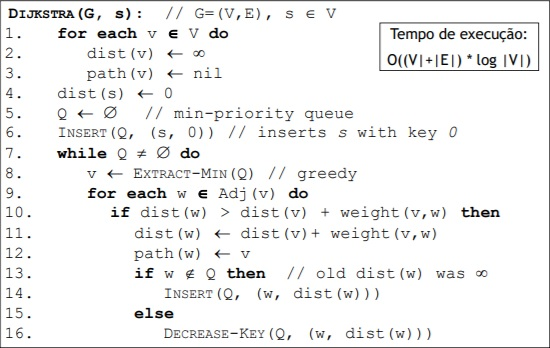
\includegraphics[scale=1]{Dijkstra_pseudocode.jpg}}
  \caption{Pseudocódigo do Algoritmo de \textit{Dijsktra}.}
\end{figure}

A utilização deste algoritmo de cálculo do caminho mais curto desde o vértice inicial (morada do utilizador) até aos outros nós (pontos de recolha) resulta numa árvore de caminhos ordenada.

A preparação do algoritmo tem complexidade temporal O($|V|$) e consiste na inicialização do campo \textbf{dist} a $\infty$ e \textbf{path} a "nil" (correspondente a \textit{nullptr}) em todos os vértices (à exceção da origem).

Posteriormente, a partir do vértice inicial, percorre-se todas as arestas adjacentes e adiciona-se os vértices de destino a uma fila de prioridade, atualizando a dist (distância do vértice anterior somada com o peso da aresta) e o path (vértice anterior), se este vértice ainda não tiver sido visitado, ou se a distância obtida for menor do que o valor prévio de dist.

Este processo tem complexidade temporal O($(|V| + |E|)*log(|V|)$), uma vez que a cada passo - O($|V| + |E|$) - pode ser necessário adicionar, remover ou mover elementos na fila de prioridade - O($log(|V|)$).
	
Para o segundo caso, ter-se-ia de aplicar uma "translação" ao mesmo algoritmo (uma vez que não se teria de calcular a distância de um nó a todos os outros, mas de um potencial ponto interno da aresta até um potencial ponto interno de outra aresta), tendo que, para todas as distâncias calculadas a partir de cada uma das extremidades dessa aresta (pelo algoritmo referido), somar-se a distância do ponto interno a essa mesma extremidade.

Posteriormente, para implementar a especificidade dos resíduos, seria apenas necessário, em cada ponto de recolha, guardar o(s) tipo(s) de resíduos nele recolhidos.

Após essa implementação, resta ter em consideração o fator capacidade, a ser guardado também em cada ponto de recolha e para cada um dos resíduos recolhidos.

\section{Novo Modelo de Negócio}

O processamento do novo modelo de negócio proposto baseia-se no cálculo do itinerário mais curto partindo da morada do utilizador e destinado a uma central de reciclagem, passando por todas as casas que desejam ver esse tipo de resíduo recolhido.

Este problema assemelha-se ao \textbf{\textit{Travelling Salesman Problem} (TSP)}, pelo que os métodos a aplicar serão semelhantes às resoluções propostas. As três opções ponderadas consistem em:

\begin{itemize}
\item \textbf{Algoritmo de Held-Karp:} Este é um algoritmo de programação dinâmica baseado em \textbf{\textit{COMPLETAR!!!}}.

\item \textbf{Algoritmo do Vizinho mais Próximo:} Este algoritmo baseia-se na ordenação dos pontos, encontrando o ponto não visitado mais próximo do anterior processado. Este algoritmo não garante um resultado ótimo, mas tem complexidade bastante inferior ao anterior (complexidade temporal O($|V|^2$) no pior caso).

\item \textbf{Força bruta:} Esta alternativa consiste no cálculo de todas as opções possíveis e seleção da mais rentável. Obviamente, este é o método mais temporalmente complexo (O($|V|!$)) e, portanto, apesar de garantir um resultado ótimo, é pouco recomendável.
\end{itemize}


\newpage

\newpage
%----------------------------------------------------------------------------------------
%	CHAPTER 4 - CASOS DE UTILIZAÇÃO
%----------------------------------------------------------------------------------------
\chapter[Casos de Utilização][Casos de Utilização]{Casos de Utilização} \label{\thechapter}

A aplicação \textit{Wasteapp} que vamos implementar terá como base uma interface simples de texto com a qual o utilizador poderá interagir. Deste modo, para facilitar a interação, esta terá um conjunto de menus com várias opções a serem disponibilizadas, dividindo-se em 2 menus gerais: 1 menu para o utilizador comum que procura os pontos de recolha mais próximos e 1 menu para o utilizador que irá explorar financeiramente o novo modelo de negócio.
Para além disso, será possível guardar a informação de um mapa sob a forma de um grafo através da leitura de ficheiros de texto, no qual incidirão as diferentes funcionalidades da \textit{app}, dentro das quais se destacam:

\begin{itemize}
\item Visualização dos dados do grafo e da informação representada por este (vias de trânsito, pontos de recolha, etc.) no \textit{GraphViewer};
\item Ordenação dos pontos de recolha por proximidade ao utilizador e do itinerário ótimo para o modelo de negócio;
\item Consulta da informação sobre os pontos de recolha disponíveis(capacidade e tipo de resíduo);
\item Verificação da acessibilidade dos pontos de recolha (verificação se as ruas se encontram desimpedidas, sem estarem em obras, por exemplo);
\item Ordenação e atribuição das casas dos utilizadores que solicitaram a recolha de resíduos ao domicílio.

\end{itemize}

\begin{figure}[h!]
  \centerline{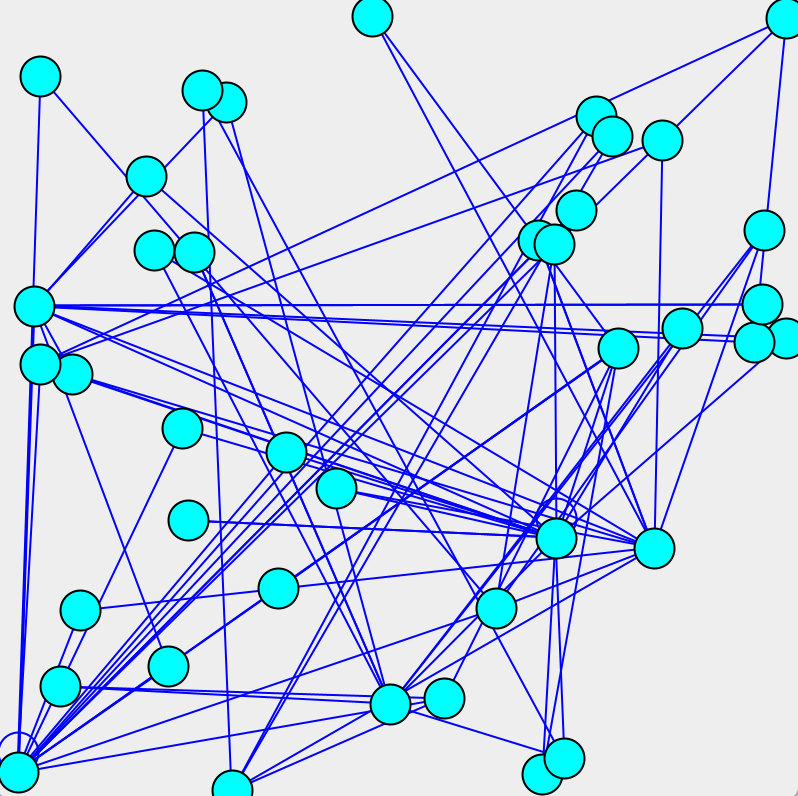
\includegraphics[scale=0.6]{graphviewer.png}}
  \caption{Exemplo de um grafo visualizado no \textit{GraphViewer}.}
\end{figure}


\newpage
%----------------------------------------------------------------------------------------
%	CHAPTER 5 - CONCLUSÃO
%----------------------------------------------------------------------------------------
\chapter[Conclusão][Conclusão]{Conclusão} \label{\thechapter}

Após um estudo rigoroso do problema que nos foi atribuído, percebemos que existem diversas maneiras para resolver problemas deste género. Depois do aconselhamento por parte da professora das aulas práticas e dos monitores, acreditamos que obtivemos uma abordagem correta para a solução do problema de identificação dos itinerários ótimos.

A nosso ver, a parte que requereu mais tempo foi o ponto a "Perspetiva de Solução" uma vez que necessitou de bastante pesquisa em diversas plataformas de forma a encontrarmos o algoritmo mais apropriado para a solução dos problemas que surgiram, pois serão utilizados diferentes algoritmos tanto na utilização "normal" da aplicação como na perspetiva de novo modelo de negócio que surge com esta.

Por fim, podemos concluir que, após a realização deste relatório, dominamos agora a matéria lecionada em aula que incide na manipulação de grafos com algoritmos, encontrando-nos, assim, preparados para a implementação do que sugerimos na parte do trabalho que se segue.
\Repeat{2}{\linebreak}

\textbf{Beatriz Costa Silva Mendes} - up201806551@fe.up.pt

Tarefas:
\begin{itemize}
\item Descrição do Tema;
\item Casos de Utilização;
\item Colaboração na Perspetiva de Solução.
\end{itemize}

\textbf{Daniel Garcia Lima Sarmento da Silva} - up201806524@fe.up.pt

Tarefas:
\begin{itemize}
\item Formalização do Problema
\end{itemize}

\textbf{Henrique Manuel Ruivo Pereira} - up201806538@fe.up.pt

Tarefas:
\begin{itemize}
\item Colaboração na Descrição do Tema;
\item Colaboração nos Casos de Utilização;
\item Perspetiva de Solução.
\end{itemize}





\newpage
%----------------------------------------------------------------------------------------
%	CHAPTER 6 - REFERÊNCIAS BIBLIOGRÁFICAS
%----------------------------------------------------------------------------------------
\chapter[Referências Bibliográficas][Referências Bibliográficas]{Referências Bibliográficas} \label{\thechapter}
Grupo B, Turma 6, 2016. \textit{Ecoponto: Recolha De Lixo Seletiva (Tema 4) ‐ Parte 1}. Projeto de Concepção e Análise de Algoritmos.

[1]: Docs.google.com. 2020. 2019-20 2S CAL Trabalhos Publicados. Disponível no Moodle.

[2]: Wikipedia Contributors (2019). \textit{Held–Karp algorithm}. [online] Wikipedia. Disponível em: \url{https://en.wikipedia.org/wiki/Held%E2%80%93Karp_algorithm}.

[3]: Wikipedia Contributors (2019). \textit{Travelling salesman problem}. [online] Wikipedia. Disponível em: \url{https://en.wikipedia.org/wiki/Travelling_salesman_problem}.

Figura 1: Rossetti, R., Ferreira, L., Cardoso, H. L. e Andrade, F., 2020. \textit{Algoritmos Em Grafos: Caminho Mais Curto (Parte I)}.

Figura 2: GitHub. (2020). \textit{STEMS-group/GraphViewer}. [online] Disponível em: \url{https://github.com/STEMS-group/GraphViewer}.

‌

‌

\newpage
\end{document}
